In this section, we provide the necessary background from a control theory perspective to facilitate the understanding of the remainder of this work. Initially, we introduce general concepts related to optimization problems. Subsequently, we delve into the foundational principles of Nonlinear Programming (NLP), with a focus on Nonlinear Model Predictive Control (NMPC) and its application within control loops. Finally, we explore the concept of cooperative control and its relevance to multi-agent systems.

\subsection{Optimization Problems}

An optimization problem is defined as the task of determining the best, or optimal, solution among all feasible solutions while adhering to a set of constraints. This process typically involves minimizing an objective function, often referred to as the cost function in specific applications. For cases where maximization is desired, the problem can be reformulated to minimize the negative of the cost function.

The general formulation of an optimization problem is presented in Equation \ref{eq:optimization_problem}, where \( f(x) \) is the cost function, \( x \) represents the decision variables, \( e_i(x) \) denotes equality constraints, and \( g_j(x) \) signifies inequality constraints. This formulation employs hard constraints, meaning that all constraints must be satisfied at all times. However, rigid enforcement of hard constraints can render the problem infeasible under certain conditions. To address this, soft constraints can be introduced by augmenting the cost function with penalty terms, as shown in Equation \ref{eq:optimization_problem_with_soft_constraint}. Here, \( sc(x) \) represents the penalty for constraint violation.

\begin{minipage}[t]{0.45\textwidth}
    \begin{equation}
        \begin{aligned}
            &\underset{x}{\text{minimize}} \quad f(x) \\
            &\text{subject to} \quad e_i(x) = 0, \quad i = 1, \dots, m, \\
            &\quad \quad \quad \quad \, g_j(x) \geq 0, \quad j = 1, \dots, p.
        \end{aligned}
        \label{eq:optimization_problem}
    \end{equation}
\end{minipage}%
\hfill
\begin{minipage}[t]{0.45\textwidth}
    \begin{equation}
        \begin{aligned}
            &\underset{x}{\text{minimize}} \quad f(x) + sc(x) \\
            &\text{subject to} \quad e_i(x) = 0, \quad i = 1, \dots, m, \\
            &\quad \quad \quad \quad \, g_j(x) \geq 0, \quad j = 1, \dots, p.
        \end{aligned}
        \label{eq:optimization_problem_with_soft_constraint}
    \end{equation}
\end{minipage}

\subsection{Nonlinear Model Predictive Control}

Nonlinear Model Predictive Control (NMPC) is an optimization-based technique for the feedback control of nonlinear systems, incorporating system constraints \cite{grune2017nonlinearmpc}. NMPC relies on a model of the system to predict its future behavior over a predefined prediction horizon. The control input that minimizes the cost function within this horizon is calculated, and only the first control action is applied. This process is repeated iteratively.

As illustrated in Figure \ref{fig:simplified_mpc_control_loop}, NMPC operates as a closed-loop control system, using the current state of the system as an input. This ensures that any deviations from the system model are accounted for in subsequent iterations.

\begin{figure}[h]
    \centering
    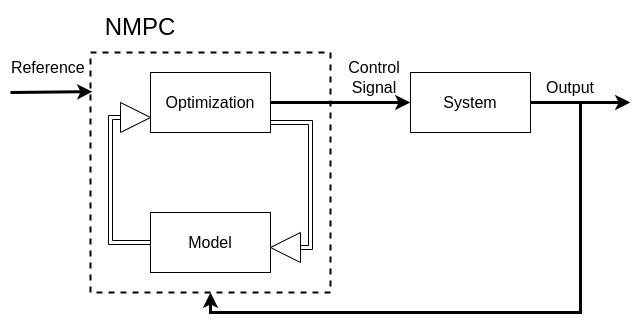
\includegraphics[width=0.8\textwidth]{Images/Background/MPC/NMPC.jpg}
    \caption{Simplified Block Diagram of an NMPC Controller}
    \label{fig:simplified_mpc_control_loop}
\end{figure}

The internal mechanism of Model Predictive Control (MPC) systems, whether linear or nonlinear, follows the same fundamental principles \cite{grune2017nonlinearmpc,schwenzer2021review}. A summary of the NMPC workflow for each time step \( t = 1, 2, \dots \) is as follows:

\begin{itemize}
    \item \textbf{State Measurement:} Measure the current state of the system, \( x(s) \in \mathbb{X} \), where \( \mathbb{X} \) is the system's state space.
    \item \textbf{Optimization Problem Definition:} Formulate the optimal control problem (OCP) as shown in Equation \ref{eq:mpc_optimization_problem}, using the current system state \( x(s) \) as the initial condition \( x_0 \). In this equation, \( f \) represents the system dynamics model, and \( l \) is the cost function to be minimized:
    \begin{equation}
        \begin{aligned}
            &\underset{u(\cdot) \in  \mathbb{U}^{N}(x_{0})}{\text{minimize}} \quad J_{N}(x_{0}, u(\cdot)) = \sum_{k=0}^{N-1} l(x_u(k, x_0), u(k)) \\
            &\text{subject to} \quad x_u(0, x_0) = x_0, \\
            &\quad \quad \quad \quad x_u(k+1, x_0) = f(x_u(k, x_0), u(k)).
        \end{aligned}
        \label{eq:mpc_optimization_problem}
    \end{equation}
    \item \textbf{Feedback and Update:} Use the computed NMPC feedback value \( \mu_{N}(x(n)) := u(0) \) for control until the next sampling period. Remaining control values can be discarded or used as warm-start inputs for the next optimization iteration.
\end{itemize}

NMPC systems often consider two types of horizons, as discussed in \cite{schwenzer2021review}: the \textit{prediction horizon} \( N_p \), where future system dynamics are simulated, and the \textit{control horizon} \( N_c \), where optimal control inputs are computed. For simplicity, we assume \( N_c = N_p \). If \( N_c < N_p \), the control input is held constant for the remaining steps.
